\documentclass{zjusct-beamer/zjusct}

% Metadata
\title{A First Look at the CPU Parallel Programming Framework} 
\subtitle{OpenMP \& MPI}
\author[YooLc]{Chenxiao Li (@YooLc)}
\date{\today}
\institute[ZJUSCT]{Zhejiang University Supercomputing Team}
\copyleftnotice{CC-BY 4.0}

\hypersetup{
    pdftitle={\title},
    pdfpagemode=FullScreen,
}

\begin{document}

% Set Mono and Emoji font
\setmonofont{DejaVu Sans Mono}
\setemojifont{TwemojiMozilla}

\maketitle

% Outline (Table of Contents)
\cutoc

\section{Introduction}

\begin{frame}{\emoji{thinking} Parallel Programming}
  \begin{columns}
    \begin{column}{0.4\textwidth}
      \begin{figure}
        \centering
        \includegraphics<1->[width=1\linewidth]{day8_am/img/intro1.png}
      \end{figure}
    \end{column}
    \begin{column}{0.6\textwidth}
      \begin{figure}
        \centering
        \includegraphics<2->[width=1\linewidth]{day8_am/img/intro2.png}
      \end{figure}
    \end{column}
  \end{columns}
  %\footnotetext{https://mpitutorial.com/tutorials/mpi-introduction/}

  %\footnotetext{https://www.mpi-forum.org/docs/}
\end{frame}

\begin{frame}{Shared Memory Parallel Model}
  \begin{columns}
    \begin{column}{0.35\textwidth}
      \centering \textbf{UMA}
      \begin{figure}
        \centering
        \includegraphics[width=\textwidth]{day8_am/img/UMA.png}
      \end{figure}
      \centering \textbf{U}niform \textbf{m}emory \textbf{a}ccess
    \end{column}
    \begin{column}{0.35\textwidth}
      \centering \textbf{NUMA}
      \begin{figure}
        \centering
        \includegraphics[height=0.5\textheight]{day8_am/img/NUMA.png}
      \end{figure}
      \centering \textbf{N}on-\textbf{u}niform \textbf{m}emory \textbf{a}ccess
    \end{column}
    \begin{column}{0.3\textwidth}
      \begin{figure}
        \centering
        \includegraphics[height=140pt]{day8_am/img/two-way.png}
      \end{figure}
      \centering In real world
    \end{column}
  \end{columns}
\end{frame}

\section{OpenMP}

\begin{frame}{OpenMP}
  \begin{columns}
    \begin{column}{0.6\textwidth}
      \parindent=2em
      \parbox[t]{\linewidth}{
        \textbf{OpenMP} (Open Multi-Processing) is an API that supports multi-platform shared-memory multiprocessing programming in \textbf{C, C++, and Fortran}.

        It provides a set of compiler directives, library routines, and environment variables that allow developers to specify parallel regions, tasks, and other parallelism constructs.

        \emoji{light-bulb} \textbf{OpenMP provides us an easy way to transform serial programs into parallel.}
      }
    \end{column}
    \begin{column}{0.4\textwidth}
      \begin{figure}
        \centering
        \includegraphics[width=1\linewidth]{day8_am/img/omp.png}
      \end{figure}
    \end{column}
  \end{columns}
\end{frame}

\begin{frame}[fragile]{Example 1: Hello OpenMP}
  \begin{columns}[T] % align columns at top
    \begin{column}{0.6\textwidth}
      \vspace{-10pt} % Align minted to the top
      \begin{minted}[fontsize=\scriptsize]{c}
#include <stdio.h>
#include <omp.h>
int main() {
  printf("Welcome to OpenMP!\n");
  #pragma omp parallel
  {
    int ID = omp_get_thread_num();
    printf("hello(%d)", ID);
    printf("world(%d)\n", ID);
  }
  printf("Bye!");
  return 0;
}
      \end{minted}
    \end{column}
    \begin{column}{0.4\textwidth}
      \emoji{crystal-ball} Output:
      \vfill
      \begin{figure}
        \centering
        \includegraphics[width=1\linewidth]{day8_am/img/example-1-output.png}
      \end{figure}
    \end{column}
  \end{columns}

  \begin{minted}[fontsize=\scriptsize,escapeinside=@@]{bash}
       $ gcc -o hello_omp hello_omp.c @-fopenmp@ # <-- Compiler Option
   \end{minted}
\end{frame}

\begin{frame}[fragile]{Example 1: Hello OpenMP}
  \begin{columns}[T] % align columns at top
    \begin{column}{0.6\textwidth}
      \vspace{-10pt} % Align minted to the top
      \begin{minted}[fontsize=\small,highlightlines={2,5,7-9},highlightcolor=Khaki1]{c}
#include <stdio.h>
#include <omp.h>
int main() {
  printf("Welcome to OpenMP!\n");
  #pragma omp parallel
  {
    int ID = omp_get_thread_num();
    printf("hello(%d)", ID);
    printf("world(%d)\n", ID);
  }
  printf("Bye!");
  return 0;
}
      \end{minted}
    \end{column}
    \begin{column}{0.4\textwidth}
      \vspace{2pt}
      \textbf{Differences:}
      \begin{itemize}
        \item \textbf<1>{Import OpenMP Header}
              \vspace{2.2em}
        \item \textbf<2>{Preprocessing directive}
              \begin{itemize}
                \item<2-> \textbf<2>{Will cover commonly used directives}
              \end{itemize}
        \item \textbf<3>{Parallel Region}
              \begin{itemize}
                \item<3> Relates to the \textbf<3>{fork-join} model
              \end{itemize}
      \end{itemize}
    \end{column}
  \end{columns}
\end{frame}

\begin{frame}[fragile]{Fork-Join Model}
  \begin{columns}[T] % align columns at top
    \begin{column}{1\textwidth}
      \vspace{-5pt}
      \begin{figure}
        \centering
        \includegraphics[width=1\linewidth]{day8_am/img/fork-join2.png}
      \end{figure}
    \end{column}
  \end{columns}
\end{frame}

\begin{frame}[fragile]{Fork-Join Model}
  \begin{columns}[T] % align columns at top
    \begin{column}{1\textwidth}
      Thread ID: \verb|omp_get_thread_num()|
      \vspace{-5pt}
      \begin{figure}
        \centering
        
\includegraphics[width=0.7\linewidth]{day8_am/img/fork-join-mine.png}
      \end{figure}
    \end{column}
  \end{columns}
\end{frame}


\subsection{OpenMP directives and constructs}

\begin{frame}[fragile]{OpenMP Directives}

  \begin{block}{A legal OpenMP Directive must has the following format (C/C++):}
    \begin{tabular}{|c|c|c|c|}
      \hline
      Pragma       & Directive                       & [clause[ [,]clause] ... ] \\
      \hline
      \#pragma omp & parallel, atomic, critical, ... & 0 to many                 \\
      \hline
    \end{tabular}
  \end{block}
  \begin{itemize}
    \item \emoji{chestnut} \textbf{For example:}
          \vspace{-5pt}
          \begin{minted}[fontsize=\scriptsize]{c}
#pragma omp parallel for collapse(2) private(tmp_v, d, v)
    \end{minted}
    \item Case sensitive
    \item Affects the block (single statement or wrapped by \verb|{}|) after this directive
    \item \emoji{zany-face} Here's an official \href{https://www.openmp.org/wp-content/uploads/OpenMPRefCard-5-2-web.pdf}{\textbf{Cheet Sheet}}
  \end{itemize}
\end{frame}

\begin{frame}[fragile]{Constructs}
  \emoji{thinking} What is the difference between \textbf{construct} and \textbf{directive}?

  \emoji{nerd-face} An OpenMP construct is a formation for which the directive is executable.\footnote{https://www.openmp.org/spec-html/5.2/openmpse14.html}

  \begin{minted}[fontsize=\small,highlightlines={5},highlightcolor=Khaki1]{c}
#pragma omp parallel    // <--\--- Directive
{                       //     |
    printf("Do sth.");  //     | Construct
}                       // ---/
\end{minted}

\end{frame}

\begin{frame}{Work-distribution constructs}
  \begin{columns}[T]

    \begin{column}{0.7\textwidth}
      \begin{figure}
        \centering
        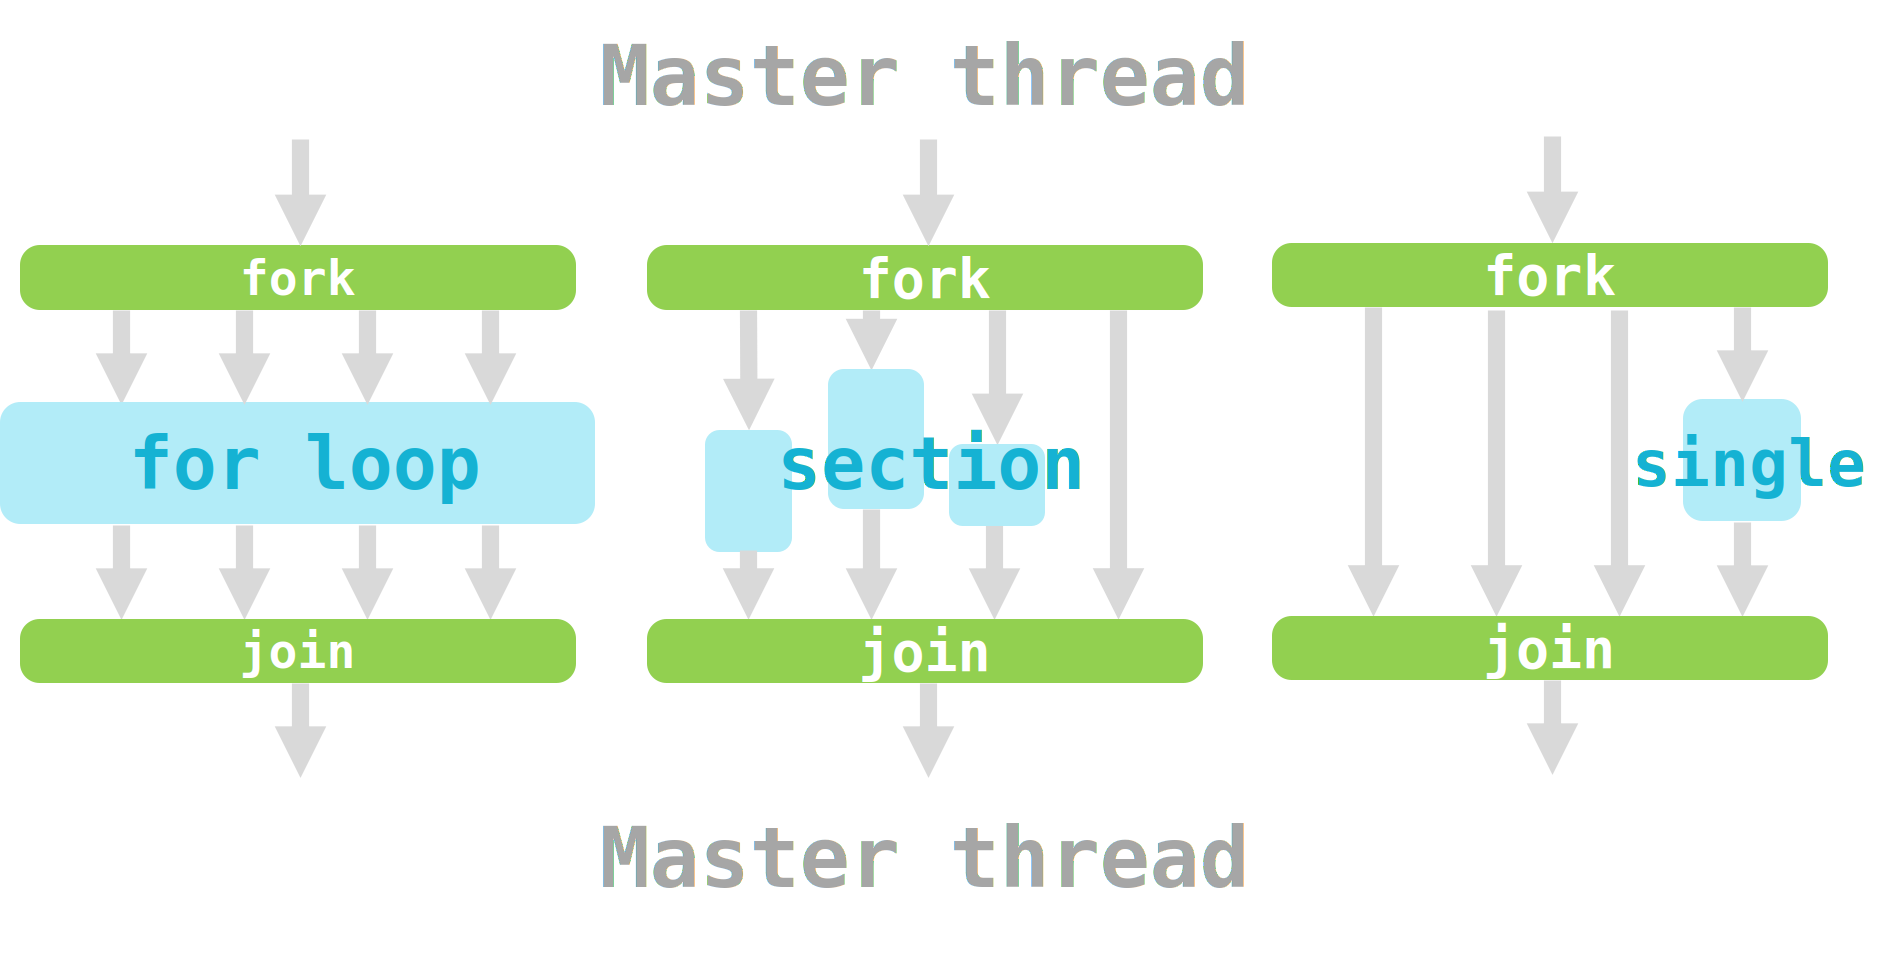
\includegraphics[width=1\linewidth]{day8_am/img/Work-distribution.png}
      \end{figure}
    \end{column}

    \begin{column}{0.3\textwidth}
      \vspace{2em}
      Work-distribution constructs:
      \begin{itemize}
        \item \textbf<1>{single}
        \item \textbf<2>{section}
        \item \textbf<3>{for}
      \end{itemize}
    \end{column}

  \end{columns}
\end{frame}

\begin{frame}[fragile]{\textit{parallel} Directive}
  \vspace{-10pt} % Align minted to the top
  \begin{minted}[fontsize=\small,highlightlines={5},highlightcolor=Khaki1]{c}
#include <stdio.h>
#include <omp.h>
int main() {
  printf("Welcome to OpenMP!\n");
  #pragma omp parallel
  {
    int ID = omp_get_thread_num();
    printf("hello(%d)", ID);
    printf("world(%d)\n", ID);
  }
  printf("Bye!");
  return 0;
}
      \end{minted}
\end{frame}

\begin{frame}[fragile]{Combined Constructs and Directives}
  \textbf{Example 2: \textit{parallel for} Directive}
  \begin{columns}[T] % align columns at top
    \begin{column}{0.5\textwidth}
      \vspace{-10pt} % Align minted to the top
      \begin{minted}[fontsize=\scriptsize]{c}
// Addition of two vectors
for (int i = 0; i < N; i++) {
    c[i] = a[i] + b[i];
}
      \end{minted}
    \end{column}

    \begin{column}{0.5\textwidth}
      \vspace{-10pt} % Align minted to the top
      \begin{minted}[fontsize=\scriptsize, highlightlines={2}]{c}
// Addition of two vectors
#pragma omp parallel for
for (int i = 0; i < N; i++) {
    c[i] = a[i] + b[i];
}
      \end{minted}
    \end{column}
  \end{columns}
  \begin{figure}
    \centering
    \includegraphics<1-2>[width=0.55\linewidth]{day8_am/img/parallel-for-1.png}
  \end{figure}
  \centering \uncover<2>{\emoji{exploding-head} Not 4x speed up}

  \uncover<3>{\emoji{hugging-face} \textbf{Overhead}: any combination of excess or indirect computation time, memory, bandwidth, or other resources that are required to perform a specific task.}
\end{frame}

\begin{frame}[fragile]{Loop Schedule}


  \begin{minted}[fontsize=\scriptsize]{c}
#pragma omp parallel for
for (int i = 0; i < N; i++) {
    c[i] = f(i); // What if f is not O(1)
}
\end{minted}

  Workload is unbalanced!

\end{frame}

\begin{frame}[fragile]{Loop Schedule}
  \begin{figure}
    \centering
    \includegraphics[width=0.8\linewidth]{day8_am/img/schedule-trace.png}
  \end{figure}

  \centering
  Static, Dynamic, Guided, Runtime, Auto

\end{frame}

\begin{frame}[fragile]{Loop Schedule - Static}

  \begin{minted}[fontsize=\scriptsize]{c}
#pragma omp parallel for schedule(static)
for (int i = 0; i < N; i++) {
    c[i] = f(i);
}
\end{minted}

  Static, Dynamic, Guided, Auto
\end{frame}

\begin{frame}[fragile]{Loop Schedule - Dynamic}

  \begin{minted}[fontsize=\scriptsize]{c}
#pragma omp parallel for schedule(dynamic, 2)
for (int i = 0; i < N; i++) {
    c[i] = f(i); // What is f is O(N^2)
}
\end{minted}

  \begin{itemize}
    \item[\emoji{thumbs-up}] Pros: More flexible scheduling
    \item[\emoji{thumbs-down}] Cons: More overhead in scheduling
  \end{itemize}

\end{frame}

\begin{frame}[fragile]{Nested \textit{for} Loop}
  \begin{columns}[T] % align columns at top
    \begin{column}{0.5\textwidth}
      \vspace{-10pt} % Align minted to the top
      \begin{minted}[fontsize=\scriptsize]{c}
// Matrix Element-wise Addition
#pragma omp parallel for
for (int i = 0; i < n; i++) {
    for (int j = 0; j < n; j++) {
        c[i][j] = a[i][j] + b[i][j];
    }
}
      \end{minted}
    \end{column}

    \begin{column}{0.5\textwidth}
      \vspace{-10pt} % Align minted to the top
      \begin{minted}[fontsize=\scriptsize, highlightlines={1}]{c}
#pragma omp parallel for collapse(2)
for (int i = 0; i < n; i++) {
    for (int j = 0; j < n; j++) {
        c[i][j] = a[i][j] + b[i][j];
    }
}
      \end{minted}
    \end{column}
  \end{columns}
\end{frame}
\subsection{Shared Data and Data Hazards}

\begin{frame}[fragile]{Example: Data Hazards in Summation}
\begin{minted}[fontsize=\scriptsize]{c}
#include <stdio.h>
#include "omp.h"
int main() {
    int a[100];
    int sum = 0;
    // initialize
    for (int i = 0; i < 100; i++) a[i] = i + 1;
    // Sum up from 1 to 100
#pragma omp parallel for
    for (int i = 0; i < 100; i++) {
        sum += a[i];
    }
    printf("Sum = %d\n", sum);
}
\end{minted}
\end{frame}

\begin{frame}[fragile]{How Data Hazards Happen?}
\begin{columns}[T]
    \begin{column}{0.7\textwidth}
        \begin{figure}
            \centering
            \includegraphics[width=\textwidth]{day8_am/img/hazard_illustration.png}
        \end{figure}
    \end{column}
    \begin{column}{0.3\textwidth}
        \begin{figure}
            \centering
            \includegraphics[width=\textwidth]{day8_am/img/hazard_schedule.png}
        \end{figure}
    \end{column}
\end{columns}
\end{frame}

\begin{frame}[fragile]{Scope and Data Hazard}
\begin{columns}[T]
    \begin{column}{0.5\textwidth}
        \begin{itemize}
            \item Shared \& private data in default
            \item Explicit scopes definition
            \begin{itemize}
                \item \textit{private}
                \item \textit{shared}
                \item \textit{firstprivate}
                \item \textit{lastprivate}
            \end{itemize}
            \item Data hazards happen when operating shared data
        \end{itemize}
    \end{column}
    \begin{column}{0.5\textwidth}
        \begin{minted}[fontsize=\scriptsize]{c}
    int sum = 0;
    // Sum up from 1 to 100
#pragma omp parallel for
    for (int i = 0; i <= 99; i++) {
        sum += a[i];
    }
\end{minted}
    \end{column}
\end{columns}
\end{frame}

\begin{frame}[fragile]{Resolve Data Hazard}
\begin{itemize}
    \item Critical Section
    \item Atomic Operations
    \item Reduction
\end{itemize}
\end{frame}

\begin{frame}[fragile]{Example: Solution with Critical Section}
\begin{columns}[T]
    \begin{column}{0.5\textwidth}
        \begin{itemize}
            \item Only one thread can enter critical section at the same time.
            \item A critical section can contain multiple statements.
        \end{itemize}
    \end{column}
    \begin{column}{0.5\textwidth}
\begin{minted}[fontsize=\scriptsize]{c}
#pragma omp parallel for
    for (int i = 0; i < 100; i++) {
#pragma omp critical
        { sum += a[i]; }
    }
    printf("Sum = %d\n", sum);
\end{minted}
    \end{column}
\end{columns}

\end{frame}

\begin{frame}[fragile]{Example: Solution with Atomic Operation}
\begin{columns}[T]
    \begin{column}{0.5\textwidth}
        \begin{itemize}
            \item Atomic operation cannot be separated.
            \item Only can be applied to one operation
            \item Limited set of operators supported
        \end{itemize}
    \end{column}
    \begin{column}{0.5\textwidth}
\begin{minted}[fontsize=\scriptsize]{c}
#pragma omp parallel for
    for (int i = 0; i < 100; i++) {
#pragma omp atomic
        sum += a[i];
    }
    printf("Sum = %d\n", sum);
\end{minted}
    \end{column}
\end{columns}
\end{frame}

\begin{frame}[fragile]{Example: Solution with Reduction}
\begin{columns}[T]
    \begin{column}{0.45\textwidth}
        \begin{itemize}
            \item Create temporary private variables for each thread
            \item Reduce these private variables in the end
            \item Limited set of operators supported
        \end{itemize}
    \end{column}
    \begin{column}{0.55\textwidth}
\begin{minted}[fontsize=\scriptsize]{c}
#pragma omp parallel for reduction(+:sum)
    for (int i = 0; i < 100; i++) {
        sum += a[i];
    }
    printf("Sum = %d\n", sum);
\end{minted}
    \end{column}
\end{columns}
\end{frame}

\begin{frame}[fragile]{Comparison}
\begin{itemize}
    \item Critical Region: Based on locking
    \item Atomic Operation: Based on hardware atomic operations
    \item Reduction: only synchronize in the end

\end{itemize}
\end{frame}

\begin{frame}[fragile]{Another Example: GEMM}
    \begin{minted}[fontsize=\scriptsize]{c}
    // General Matrix Multiplication (GEMM)
    for (int i = 0; i < N; i++) {
        for (int j = 0; j < N; j++) {
            c[i][j] = 0;
            for (int k = 0; k < N; k++) {
                c[i][j] += a[i][k] * b[k][j];
            }
        }
    }
    \end{minted}
\end{frame}

\begin{frame}[fragile]{Another Example: GEMM}
    \begin{minted}[fontsize=\scriptsize]{c}
#pragma omp parallel for collapse(3) reduction(+ : c)
    for (int i = 0; i < N; i++) {
        for (int j = 0; j < N; j++) {
            c[i][j] = 0;
            for (int k = 0; k < N; k++) {
                c[i][j] += a[i][k] * b[k][j];
            }
        }
    }
    \end{minted}
\end{frame}
\subsection{Pitfalls \& Fallacies}

% \begin{frame}{Threads Synchronize}
%   \begin{columns}[T] % align columns at top
%     \begin{column}{0.5\textwidth}
%     \vspace{-10pt} % Align minted to the top
%     \begin{itemize}
%         \item \emoji{no-entry} Barrier: Wait until all thread reach here
%         \begin{itemize}
%             \item Implicit barrier in parallel region
%             \item \textit{nowait} clause
%         \end{itemize}
%         \item Locking: wait until obtain the lock
%         \begin{itemize}
%             \item Often apply to data structures
%         \end{itemize}
%     \end{itemize}
%     \end{column}

%     \begin{column}{0.5\textwidth}
%     \vspace{-10pt} % Align minted to the top
%     \begin{figure}
%         \centering
%         \includegraphics[width=0.5\linewidth]{day8_am/img/barrier.png}
%     \end{figure}
%     \end{column}
%   \end{columns}

% \end{frame}

\begin{frame}[fragile]{Nested Parallel Region}
    \begin{columns}[T] % align columns at top
        \begin{column}{0.3\textwidth}
            \begin{itemize}
                \item Disabled in default.
                \item Use \textit{omp\_set\_nested} to enable.
            \end{itemize}
        \end{column}

        \begin{column}{0.7\textwidth}
            \begin{minted}[fontsize=\scriptsize, highlightlines={1}]{c}
#pragma omp parallel for
for (int i = 0; i < n; i++) {
#pragma omp parallel for
    for (int j = 0; j < n; j++) {
        c[i][j] = a[i][j] + b[i][j];
    }
}
            \end{minted}
        \end{column}
    \end{columns}
\end{frame}

\begin{frame}{False Sharing}
    \begin{figure}
        \centering
        \includegraphics[width=0.5\linewidth]{day8_am/img/false_sharing.png}
    \end{figure}
\end{frame}

\begin{frame}{Takeaway: How to Optimize a program with OpenMP}
    \begin{enumerate}
        \item \textbf{Where}: Profiling
        \item \textbf{Why}: Analyze data dependency
        \item \textbf{How}: Analysis and Skills
              \begin{itemize}
                  \item Sub-task Distribution
                  \item Scheduling Strategy
                  \item Cache and Locality
                  \item Hardware Environment
              \end{itemize}
        \item Get Down to Work: Testing
    \end{enumerate}
\end{frame}

\begin{frame}{Takeaway: Tips}
    \begin{enumerate}
        \item Ensure correctness while parallelizing
        \item Be aware of overhead
        \item Check more details in official documents
    \end{enumerate}
\end{frame}

\section{Introduction}

\begin{frame}{\emoji{thinking} Parallel Programming}
  \begin{columns}
    \begin{column}{0.4\textwidth}
      \begin{figure}
        \centering
        \includegraphics<1->[width=1\linewidth]{day8_am/img/intro1.png}
      \end{figure}
    \end{column}
    \begin{column}{0.6\textwidth}
      \begin{figure}
        \centering
        \includegraphics<2->[width=1\linewidth]{day8_am/img/intro2.png}
      \end{figure}
    \end{column}
  \end{columns}
  %\footnotetext{https://mpitutorial.com/tutorials/mpi-introduction/}

  %\footnotetext{https://www.mpi-forum.org/docs/}
\end{frame}

\begin{frame}{Shared Memory Parallel Model}
  \begin{columns}
    \begin{column}{0.35\textwidth}
      \centering \textbf{UMA}
      \begin{figure}
        \centering
        \includegraphics[width=\textwidth]{day8_am/img/UMA.png}
      \end{figure}
      \centering \textbf{U}niform \textbf{m}emory \textbf{a}ccess
    \end{column}
    \begin{column}{0.35\textwidth}
      \centering \textbf{NUMA}
      \begin{figure}
        \centering
        \includegraphics[height=0.5\textheight]{day8_am/img/NUMA.png}
      \end{figure}
      \centering \textbf{N}on-\textbf{u}niform \textbf{m}emory \textbf{a}ccess
    \end{column}
    \begin{column}{0.3\textwidth}
      \begin{figure}
        \centering
        \includegraphics[height=140pt]{day8_am/img/two-way.png}
      \end{figure}
      \centering In real world
    \end{column}
  \end{columns}
\end{frame}

\section{OpenMP}

\begin{frame}{OpenMP}
  \begin{columns}
    \begin{column}{0.6\textwidth}
      \parindent=2em
      \parbox[t]{\linewidth}{
        \textbf{OpenMP} (Open Multi-Processing) is an API that supports multi-platform shared-memory multiprocessing programming in \textbf{C, C++, and Fortran}.

        It provides a set of compiler directives, library routines, and environment variables that allow developers to specify parallel regions, tasks, and other parallelism constructs.

        \emoji{light-bulb} \textbf{OpenMP provides us an easy way to transform serial programs into parallel.}
      }
    \end{column}
    \begin{column}{0.4\textwidth}
      \begin{figure}
        \centering
        \includegraphics[width=1\linewidth]{day8_am/img/omp.png}
      \end{figure}
    \end{column}
  \end{columns}
\end{frame}

\begin{frame}[fragile]{Example 1: Hello OpenMP}
  \begin{columns}[T] % align columns at top
    \begin{column}{0.6\textwidth}
      \vspace{-10pt} % Align minted to the top
      \begin{minted}[fontsize=\scriptsize]{c}
#include <stdio.h>
#include <omp.h>
int main() {
  printf("Welcome to OpenMP!\n");
  #pragma omp parallel
  {
    int ID = omp_get_thread_num();
    printf("hello(%d)", ID);
    printf("world(%d)\n", ID);
  }
  printf("Bye!");
  return 0;
}
      \end{minted}
    \end{column}
    \begin{column}{0.4\textwidth}
      \emoji{crystal-ball} Output:
      \vfill
      \begin{figure}
        \centering
        \includegraphics[width=1\linewidth]{day8_am/img/example-1-output.png}
      \end{figure}
    \end{column}
  \end{columns}

  \begin{minted}[fontsize=\scriptsize,escapeinside=@@]{bash}
       $ gcc -o hello_omp hello_omp.c @-fopenmp@ # <-- Compiler Option
   \end{minted}
\end{frame}

\begin{frame}[fragile]{Example 1: Hello OpenMP}
  \begin{columns}[T] % align columns at top
    \begin{column}{0.6\textwidth}
      \vspace{-10pt} % Align minted to the top
      \begin{minted}[fontsize=\small,highlightlines={2,5,7-9},highlightcolor=Khaki1]{c}
#include <stdio.h>
#include <omp.h>
int main() {
  printf("Welcome to OpenMP!\n");
  #pragma omp parallel
  {
    int ID = omp_get_thread_num();
    printf("hello(%d)", ID);
    printf("world(%d)\n", ID);
  }
  printf("Bye!");
  return 0;
}
      \end{minted}
    \end{column}
    \begin{column}{0.4\textwidth}
      \vspace{2pt}
      \textbf{Differences:}
      \begin{itemize}
        \item \textbf<1>{Import OpenMP Header}
              \vspace{2.2em}
        \item \textbf<2>{Preprocessing directive}
              \begin{itemize}
                \item<2-> \textbf<2>{Will cover commonly used directives}
              \end{itemize}
        \item \textbf<3>{Parallel Region}
              \begin{itemize}
                \item<3> Relates to the \textbf<3>{fork-join} model
              \end{itemize}
      \end{itemize}
    \end{column}
  \end{columns}
\end{frame}

\begin{frame}[fragile]{Fork-Join Model}
  \begin{columns}[T] % align columns at top
    \begin{column}{1\textwidth}
      \vspace{-5pt}
      \begin{figure}
        \centering
        \includegraphics[width=1\linewidth]{day8_am/img/fork-join2.png}
      \end{figure}
    \end{column}
  \end{columns}
\end{frame}

\begin{frame}[fragile]{Fork-Join Model}
  \begin{columns}[T] % align columns at top
    \begin{column}{1\textwidth}
      Thread ID: \verb|omp_get_thread_num()|
      \vspace{-5pt}
      \begin{figure}
        \centering
        
\includegraphics[width=0.7\linewidth]{day8_am/img/fork-join-mine.png}
      \end{figure}
    \end{column}
  \end{columns}
\end{frame}


\subsection{Point-to-Point Communication}

\begin{frame}[fragile]{Blocking Send and Receive}
\begin{columns}
    
\begin{column}{.42\textwidth}
\begin{tabular}{c}
      \begin{minted}[fontsize=\footnotesize]{c}
int MPI_Send(
    const void* buffer,
    int count,
    MPI_Datatype datatype,
    int recipient,
    int tag,
    MPI_Comm communicator);    
      \end{minted}
\end{tabular}
\end{column}

\begin{column}{.58\textwidth}
\textbf{\large Parameters:}

\begin{itemize}
    \item \textbf{buffer} The buffer to send.

    \item \textbf{count} The number of elements to send.

    \item \textbf{datatype} The type of one buffer element.

    \item \textbf{recipient} The rank of the recipient MPI process.

    \item \textbf{tag} The tag to assign to the message.

    \item \textbf{communicator} The communicator in which the standard send takes place.
\end{itemize}

\end{column}
\end{columns}
\end{frame}

\begin{frame}[fragile]{Blocking Send and Receive}
\begin{columns}
    
\begin{column}{.4\textwidth}
\begin{tabular}{c}
    \begin{minted}[fontsize=\footnotesize]{c}
int MPI_Recv(
    void* buffer,
    int count,
    MPI_Datatype datatype,
    int sender,
    int tag,
    MPI_Comm communicator,
    MPI_Status* status);
      \end{minted}
\end{tabular}
\end{column}

\begin{column}{.6\textwidth}
\textbf{\large Parameters:}
{\footnotesize
\begin{itemize}
    \item \textbf{buffer} The buffer to receive.

    \item \textbf{count} The number of elements to receive.

    \item \textbf{datatype} The type of one buffer element.

    \item \textbf{sender} The rank of the sender MPI process.

    \item \textbf{tag} The tag to assign to the message.

    \item \textbf{communicator} The communicator in which the standard receive takes place.

    \item \textbf{status} The variable in which store the status of the receive operation. Pass MPI\_STATUS\_IGNORE if unused.
\end{itemize}
}
\end{column}
\end{columns}
\end{frame}

\begin{frame}{MPI\_Status}
    MPI\_Status represents the status of a reception operation.

    At least 3 attributes: 
    \begin{itemize}
        \item MPI\_SOURCE
        \item MPI\_TAG
        \item MPI\_ERROR
    \end{itemize}

    There may be additional attributes that are implementation-specific.
\end{frame}

\begin{frame}{Message Envelope}
    In addition to the data part, messages carry information that can be used to distinguish messages and selectively receive them.
    \begin{itemize}
        \item source
        \item destination
        \item tag
        \item communicator
    \end{itemize}
\end{frame}


\begin{frame}{Communication Mode}
\only<1>{
    \begin{itemize}
        \item \textbf{Buffer Mode}
        
        Can be started whether or not a matching receive was posted.
        Completion does not depend on the occurrence of a matching receive.
        \item \textbf{Synchronous Mode}

        Can be started whether or not a matching receive was posted.

        The send will be completed successfully only if a matching receive is posted.

        \item \textbf{Ready Mode}

        May be started only if the matching receive is already posted.

        \item \textbf{Standard Mode}

        Depends.
        
    \end{itemize}
}

\only<2>{
\footnotesize

    \begin{table}[]
\begin{tabular}{lll}

\textbf{Communication mode} & \textbf{Start time}   & \textbf{Completion time}                         \\
\hline
Buffer mode        & Immediately                 & Message has gone to buffer              \\
\hline
Synchronous mode   & Immediately                 & Matching receive has posted \\
\hline
Ready mode         & Matching receive has posted & When the send buffer can be reused      \\
\hline
Standard mode      & Depends                     & Depends  \\                  \hline      

\end{tabular}


\end{table}
}
\end{frame}

\begin{frame}[fragile]{Communication mode: A common mistake}

    \textbf{Note}: MPI\_Ssend will \textbf{always wait until the receive has been posted} on the receiving end.
    \begin{minted}[fontsize=\footnotesize]{c}
// n = 2
MPI_Comm_rank(comm, &my_rank);
MPI_Ssend(sendbuf, count, MPI_INT, my_rank ^ 1, tag, comm);
MPI_Recv(recvbuf, count, MPI_INT, my_rank ^ 1, tag, comm, &status);
      \end{minted}

    \onslide<1->{\emoji{thinking} What will happen?}

    \onslide<2>{\emoji{exploding-head} Deadlock! Any solutions?}
\end{frame}

\begin{frame}[fragile]{Communication mode: Solution}
    \begin{tabular}{c}
      \begin{minted}[fontsize=\footnotesize]{c}
// n = 2
MPI_Comm_rank(comm, &my_rank);
if (my_rank == 0) {
    MPI_Ssend(sendbuf, count, MPI_INT, 1, tag, comm);
    MPI_Recv(recvbuf, count, MPI_INT, 1, tag, comm, &status);
} else if (my_rank == 1) {
    MPI_Recv(recvbuf, count, MPI_INT, 0, tag, comm, &status);
    MPI_Ssend(sendbuf, count, MPI_INT, 0, tag, comm);
}
      \end{minted}
    \end{tabular}

    \onslide<2->{\emoji{thinking} Any other solutions?}
\end{frame}

\begin{frame}[fragile]{Blocking Send and Receive}
\begin{columns}
    
\begin{column}{.5\textwidth}
\begin{minted}[fontsize=\footnotesize]{c}
int MPI_Sendrecv(
    const void* buffer_send,      
    int count_send,
    MPI_Datatype datatype_send,
    int recipient,
    int tag_send,
    void* buffer_recv,
    int count_recv,
    MPI_Datatype datatype_recv,
    int sender,
    int tag_recv,
    MPI_Comm communicator,
    MPI_Status* status);
\end{minted}
\end{column}

\begin{column}{.5\textwidth}
\begin{block}{Notice}
    The buffers used for send and receive must be different.
\end{block}

\onslide<2->{\emoji{thinking} Any other solutions?}

\end{column}
\end{columns}
\end{frame}

\begin{frame}[fragile]{Non-Blocking Send and Receive}
\begin{block}{Recall}
    A nonblocking call initiates the operation,
    but does not complete it.
    
    They will return almost immediately.
\end{block}
    
\begin{minted}[fontsize=\footnotesize]{c}
int MPI_Isend(const void* buffer,
              int count,
              MPI_Datatype datatype,
              int recipient,
              int tag,
              MPI_Comm communicator,
              MPI_Request* request);
\end{minted}
\end{frame}

\begin{frame}{Synchronization}
    \begin{columns}
        \begin{column}{.5\textwidth}
        
            \begin{itemize}
                \item \textbf{MPI\_Test}

                MPI\_TEST(request, flag, status)
                
                \begin{itemize}

                \item Checks if a non-blocking operation is complete at a given time.
                
                \item flag=true if completes.
                \end{itemize}
            \end{itemize}
        \end{column}

        \begin{column}{.5\textwidth}
            \begin{itemize}
                \item \textbf{MPI\_Wait}

                MPI\_WAIT(request, status)

                \begin{itemize}
                    \item Waits for a non-blocking operation to complete. 
                    \item That is, unlike MPI\_Test, MPI\_Wait will block until the underlying non-blocking operation completes.
                \end{itemize}
            \end{itemize}
        \end{column}
    \end{columns}
\end{frame}

\begin{frame}[fragile]{Non-Blocking Send and Receive(Deadlock revisit)}
\begin{minted}[fontsize=\footnotesize]{c}
MPI_Request req;
MPI_Isend(sendbuf, 0x100, MPI_INT, my_rank^1, 0, MPI_COMM_WORLD, &req);
MPI_Recv(recvbuf, 0x100, MPI_INT, my_rank^1, 0, MPI_COMM_WORLD, MPI_STATUS_IGNORE);
\end{minted}
\end{frame}
\subsection{Collective Communication}

\begin{frame}{Synchronization}
    \begin{columns}
        \begin{column}{.5\textwidth}
        
            \begin{itemize}
                \item \textbf{MPI\_Barrier}

                MPI\_Barrier(COMM)

                Blocks all MPI processes in the given communicator until they all call this routine.
            \end{itemize}
        \end{column}

        \begin{column}{.5\textwidth}
            \begin{figure}
                \centering
                \includegraphics[width=0.7\linewidth]{day8_am/img/mpi/barrier.png}
                \caption{MPI\_Barrier}
                \label{fig:barrier}
            \end{figure}
        \end{column}
    \end{columns}
\end{frame}

\begin{frame}[fragile]{Broadcast: One to All}
    \begin{columns}
    
\begin{column}{.4\textwidth}
\begin{minted}[fontsize=\footnotesize]{c}
int MPI_Bcast(
    void* buffer,
    int count,
    MPI_Datatype datatype,
    int emitter_rank,
    MPI_Comm communicator);
\end{minted}

{\footnotesize
\begin{itemize}
    \item \textbf{emitter\_rank} 
The rank of the MPI process that broadcasts the data, all other processes receive the data broadcasted.
\end{itemize}
}
\end{column}

\begin{column}{.6\textwidth}
\begin{figure}
    \centering
    \includegraphics[width=0.75\linewidth]{day8_am/img/mpi/bcast.png}
    \caption{Bcast}
    \label{fig:bcast}
\end{figure}
\end{column}
\end{columns}
\end{frame}

\begin{frame}[fragile]{Broadcast: One to All}
\textbf{\large Why not Send and Receive?}

\begin{minted}[fontsize=\tiny]{c}
double start = MPI_Wtime();

if(my_rank == 0){
    for(int i=1; i<=31; i++)
        MPI_Send(sendbuf, 0x10000, MPI_INT, i, 0, MPI_COMM_WORLD);
}else{
    MPI_Recv(recvbuf, 0x10000, MPI_INT, 0, 0, MPI_COMM_WORLD, MPI_STATUS_IGNORE);
}

double end = MPI_Wtime();

if(my_rank == 0) printf("[Send Recv] Finished in %f seconds\n", my_rank, end-start);

start = MPI_Wtime();
MPI_Bcast(&sendbuf, 0x10000, MPI_INT, 0, MPI_COMM_WORLD);
end = MPI_Wtime();

if(my_rank == 0) printf("[Bcast] Finished in %f seconds\n", my_rank, end-start);
\end{minted}

\end{frame}

\begin{frame}{Broadcast: Tree based algorithm}
    \begin{figure}
        \centering
        \includegraphics[width=0.65\linewidth]{day8_am/img/mpi/broadcasttree.png}
    \end{figure}
\end{frame}

\begin{frame}[fragile]{Scatter(One to All)}
    \begin{columns}
    
\begin{column}{.5\textwidth}
\begin{minted}[fontsize=\scriptsize]{c}
int MPI_Scatter(
    const void* buffer_send,
    int count_send,
    MPI_Datatype datatype_send,
    void* buffer_recv,
    int count_recv,
    MPI_Datatype datatype_recv,
    int root,
    MPI_Comm communicator);
\end{minted}

{\scriptsize
\begin{itemize}
    \item \textbf{count\_send}
    The number of elements to send to each process.

    \item \textbf{count\_receive}
    The number of elements in the receive buffer.
    
\end{itemize}
}
\end{column}

\begin{column}{.5\textwidth}
\begin{figure}
    \centering
    \includegraphics[width=0.8\linewidth]{day8_am/img/mpi/scatter.png}
    \caption{Scatter}
    \label{fig:scatter}
\end{figure}
\end{column}
\end{columns}
\end{frame}

\begin{frame}[fragile]{Gather: All to One}
    \begin{columns}
    
\begin{column}{.5\textwidth}
\begin{minted}[fontsize=\footnotesize]{c}
int MPI_Gather(
    const void* buffer_send,
    int count_send,
    MPI_Datatype datatype_send,
    void* buffer_recv,
    int count_recv,
    MPI_Datatype datatype_recv,
    int root,
    MPI_Comm communicator);
\end{minted}

\end{column}

\begin{column}{.5\textwidth}
\begin{figure}
    \centering
    \includegraphics[width=0.75\linewidth]{day8_am/img/mpi/gather.png}
    \caption{MPI\_Gather}
\end{figure}
\end{column}
\end{columns}
\end{frame}

\begin{frame}[fragile]{Scatter and Gather}
    \begin{example}
        \textbf{Compute average}
    \end{example}
     \begin{minted}[fontsize=\scriptsize]{c}
MPI_Scatter(buffer, 0x1000000/4, MPI_DOUBLE, local_buffer, 0x1000000/4, MPI_DOUBLE, 0, MPI_COMM_WORLD);
double local_avg = 0;
for(int i=0; i<0x1000000/4; i++){
    local_avg += local_buffer[i];
}
local_avg /= 0x1000000/4;
double avgs[4];
MPI_Gather(&local_avg, 1, MPI_DOUBLE, avgs, 1, MPI_DOUBLE, 0, MPI_COMM_WORLD);
\end{minted}
\end{frame}

\begin{frame}[fragile]{Allgather(All to All)}
    \begin{columns}
    
\begin{column}{.5\textwidth}
\begin{minted}[fontsize=\footnotesize]{c}
int MPI_Allgather(
    const void* buffer_send,
    int count_send,
    MPI_Datatype datatype_send,
    void* buffer_recv,
    int count_recv,
    MPI_Datatype datatype_recv,
    MPI_Comm communicator);
\end{minted}

Actually MPI\_Gather + MPI\_Bcast.

\end{column}

\begin{column}{.5\textwidth}
\begin{figure}
    \centering
    \includegraphics[width=0.75\linewidth]{day8_am/img/mpi/allgather.png}
    \caption{MPI\_Allgather}
    \label{fig:enter-label}
\end{figure}
\end{column}
\end{columns}
\end{frame}

\begin{frame}[fragile]{Reduce}
    \begin{columns}
    
\begin{column}{.5\textwidth}
\begin{minted}[fontsize=\footnotesize]{c}
int MPI_Reduce(
    const void* send_buffer,
    void* receive_buffer,
    int count,
    MPI_Datatype datatype,
    MPI_Op operation,
    int root,
    MPI_Comm communicator);
\end{minted}

\end{column}

\begin{column}{.5\textwidth}
\begin{figure}
    \centering
    \includegraphics[width=0.75\linewidth]{day8_am/img/mpi/reduce.png}
    \caption{Reduce}
    \label{fig:reduce}
\end{figure}
\end{column}
\end{columns}
\end{frame}

\begin{frame}[fragile]{Reduce}
    \begin{example}
        \textbf{Compute average revisit}
    \end{example}
     \begin{minted}[fontsize=\scriptsize]{c}
MPI_Scatter(buffer, 0x1000000/4, MPI_DOUBLE, local_buffer, 0x1000000/4, MPI_DOUBLE, 0, MPI_COMM_WORLD);
double local_avg = 0;
for(int i=0; i<0x1000000/4; i++){
    local_avg += local_buffer[i];
}
local_avg /= 0x1000000/4;
double global_avg;
MPI_Reduce(&local_avg, &global_avg, 1, MPI_DOUBLE, MPI_SUM, 0, MPI_COMM_WORLD);
\end{minted}
\end{frame}
\subsection{Example}

\begin{frame}{Task}
\begin{columns}
    
\begin{column}{0.5\textwidth}

\scriptsize
    Implement a data validation algorithm using SHA512.
    
    Algorithm procedure:
    \begin{enumerate}
        \item Tile the input file into blocks of 1MB. (If the last block is smaller than 1MB, pad it with zeros.)
        \item For the $i^{th}$ block, concatenate it with the validation sum SHA512 of $(i-1)^{th}$ block and calculate validation sum of SHA512.
        \item The validation sum of the last block is considered as the validation sum of the entire file.
    \end{enumerate}

    \textbf{Source}: HPC Game 2024
\end{column}

\begin{column}{0.5\textwidth}
    \begin{figure}
        \centering
        \includegraphics[width=0.65\linewidth]{day8_am/img/mpi/SHA512.png}
    \end{figure}
\end{column}
\end{columns}
\end{frame}

\begin{frame}[fragile]{Baseline Code}
    \begin{columns}
    \begin{column}{.5\textwidth}
\begin{minted}[fontsize=\tiny]{c}
int num_block = (len + BLOCK_SIZE - 1) / BLOCK_SIZE;
uint8_t prev_md[SHA512_DIGEST_LENGTH];

EVP_MD_CTX *ctx = EVP_MD_CTX_new();
EVP_MD *sha512 = EVP_MD_fetch(nullptr, "SHA512", nullptr);

SHA512(nullptr, 0, prev_md);
\end{minted}
        \end{column}
        
        \begin{column}{.5\textwidth}
        \begin{minted}[fontsize=\tiny]{c}
for (int i = 0; i < num_block; i++) {
    uint8_t buffer[BLOCK_SIZE]{};
    EVP_DigestInit_ex(ctx, sha512, nullptr);
    std::memcpy(buffer, data + i * BLOCK_SIZE,
                std::min(BLOCK_SIZE, len - i * BLOCK_SIZE));
    EVP_DigestUpdate(ctx, buffer, BLOCK_SIZE);
    EVP_DigestUpdate(ctx, prev_md, SHA512_DIGEST_LENGTH);

    unsigned int len = 0;
    EVP_DigestFinal_ex(ctx, prev_md, &len);
}
              \end{minted}
        
        \begin{block}{\scriptsize Notice}
        \scriptsize
            EVP\_DigestUpdate(a);
            EVP\_DigestUpdate(b);
            
            Equivalent to EVP\_DigestUpdate(concate(a,b)) !
        \end{block}
        \end{column}

    \end{columns}
    
\end{frame}

\begin{frame}{Analysis}
    Computation is dependent on the result of the previous one.
    
    How to exploit MPI?

\end{frame}

\begin{frame}{Analysis}
    Computation is dependent on the result of the previous one.
    
    How to exploit MPI?

    \vspace{1cm}

    \textbf{Answer:}
    
    File \textbf{I/O} accounts! We can \textbf{overlap} I/O operations with computation.
\end{frame}

\begin{frame}[fragile]{MPI Code}
    \begin{columns}
    \begin{column}{.5\textwidth}
        \textbf{\scriptsize Non-Blocking receives the previous block's checksum.}
            \begin{minted}[fontsize=\tiny]{c}
if(i != 0) {
  MPI_Irecv((void *)prev_md,
          SHA512_DIGEST_LENGTH,
          MPI_UINT8_T,
          sender,
          0,
          MPI_COMM_WORLD,
          &request);
}
              \end{minted}
        \end{column}
        
        \begin{column}{.5\textwidth}
        \textbf{\scriptsize Meanwhile... File I/O and Digest}
                \begin{minted}[fontsize=\tiny]{c}
istrm.seekg(i * BLOCK_SIZE);
istrm.read(reinterpret_cast<char *>(data + i * BLOCK_SIZE), std::min(BLOCK_SIZE*local_size, file_size - i * BLOCK_SIZE));

for(int j=i; j<upper_bound; j++){
    uint8_t buffer2[BLOCK_SIZE]{};
    EVP_DigestInit_ex(ctx[j-i], sha512, nullptr);
    std::memcpy(buffer2, data + j * BLOCK_SIZE,
                std::min(BLOCK_SIZE, len - j * BLOCK_SIZE));
    EVP_DigestUpdate(ctx[j-i], buffer2, BLOCK_SIZE);
}

if(i != 0){
    MPI_Wait(&request, MPI_STATUS_IGNORE);
}
              \end{minted}
        \end{column}
        
    \end{columns}
    
\end{frame}

\begin{frame}[fragile]{MPI Code (cont.)}
    \begin{columns}
    \begin{column}{.45\textwidth}
        \textbf{\scriptsize Non-blocking send my checksum}
        \begin{minted}[fontsize=\tiny]{c}
unsigned int len = 0;
for(int j=i; j<upper_bound; j++){
    EVP_DigestUpdate(ctx[j-i], prev_md, SHA512_DIGEST_LENGTH);
    EVP_DigestFinal_ex(ctx[j-i], prev_md, &len);
}
if(upper_bound != num_block) {
    MPI_Isend(prev_md,
        SHA512_DIGEST_LENGTH,
        MPI_UINT8_T,
        recepient,
        0,
        MPI_COMM_WORLD,
        &request);
}
              \end{minted}
        \end{column}
        
        \begin{column}{.55\textwidth}
        \begin{figure}
            \centering
            \includegraphics[width=1.0\linewidth]{day8_am/img/mpi/speedup.png}
        \end{figure}

        \vspace{0.5cm}

        \end{column}
        
    \end{columns}
    
\end{frame}

\begin{frame}{Wrap up}
    \begin{figure}
            \centering
            \includegraphics[width=0.45\linewidth]{day8_am/img/mpi/SHA512para.png}
    \end{figure}
\end{frame}

\subsection{Pitfalls \& Fallacies}

% \begin{frame}{Threads Synchronize}
%   \begin{columns}[T] % align columns at top
%     \begin{column}{0.5\textwidth}
%     \vspace{-10pt} % Align minted to the top
%     \begin{itemize}
%         \item \emoji{no-entry} Barrier: Wait until all thread reach here
%         \begin{itemize}
%             \item Implicit barrier in parallel region
%             \item \textit{nowait} clause
%         \end{itemize}
%         \item Locking: wait until obtain the lock
%         \begin{itemize}
%             \item Often apply to data structures
%         \end{itemize}
%     \end{itemize}
%     \end{column}

%     \begin{column}{0.5\textwidth}
%     \vspace{-10pt} % Align minted to the top
%     \begin{figure}
%         \centering
%         \includegraphics[width=0.5\linewidth]{day8_am/img/barrier.png}
%     \end{figure}
%     \end{column}
%   \end{columns}

% \end{frame}

\begin{frame}[fragile]{Nested Parallel Region}
    \begin{columns}[T] % align columns at top
        \begin{column}{0.3\textwidth}
            \begin{itemize}
                \item Disabled in default.
                \item Use \textit{omp\_set\_nested} to enable.
            \end{itemize}
        \end{column}

        \begin{column}{0.7\textwidth}
            \begin{minted}[fontsize=\scriptsize, highlightlines={1}]{c}
#pragma omp parallel for
for (int i = 0; i < n; i++) {
#pragma omp parallel for
    for (int j = 0; j < n; j++) {
        c[i][j] = a[i][j] + b[i][j];
    }
}
            \end{minted}
        \end{column}
    \end{columns}
\end{frame}

\begin{frame}{False Sharing}
    \begin{figure}
        \centering
        \includegraphics[width=0.5\linewidth]{day8_am/img/false_sharing.png}
    \end{figure}
\end{frame}

\begin{frame}{Takeaway: How to Optimize a program with OpenMP}
    \begin{enumerate}
        \item \textbf{Where}: Profiling
        \item \textbf{Why}: Analyze data dependency
        \item \textbf{How}: Analysis and Skills
              \begin{itemize}
                  \item Sub-task Distribution
                  \item Scheduling Strategy
                  \item Cache and Locality
                  \item Hardware Environment
              \end{itemize}
        \item Get Down to Work: Testing
    \end{enumerate}
\end{frame}

\begin{frame}{Takeaway: Tips}
    \begin{enumerate}
        \item Ensure correctness while parallelizing
        \item Be aware of overhead
        \item Check more details in official documents
    \end{enumerate}
\end{frame}

% Q&A
\begin{frame}[standout]
    \Huge\textsc{Thank You}
    \vfill
    \LARGE\textsc{Any Questions?}
\end{frame}

\end{document}